\section{Обзор}
\subsection{Символьное исполнение}
Символьное исполнение --- это подход исполнения программ, который использует символьные значения вместо конкретных и исполняет множество путей исполнения программы вместо одного, как при стандартном исполнении. Например, ($x$, $y$, $z$, \dots) вместо ($17$, $``cat''$, $true$, \dots). 

\begin{lstlisting}[caption={Программа для иллюстрации символьного исполнения},captionpos=b,label={baldoni_listing}]
void foobar(int a, int b)
{
    int x = 1, y = 0;
    if (a != 0) {
        y = 3+x;
        if (b == 0)
            x = 2*(a+b);
    }
    assert(x-y != 0);
}
\end{lstlisting}
На листинге~\ref{baldoni_listing} представлен фрагмент кода, взятый из работы~\cite{baldoni2018survey}.
Цель символьного исполнения --- найти все входы программы, а именно значения переменных $a$ и $b$, для которых не выполнится <<assert>>. Полный перебор не применим, поскольку каждая переменная может принимать $2^{32}$ значений.
Эту проблему и пытается решить символьное исполнение, заменяя начальные значения переменных $a$ и $b$ на символьные $\alpha$ и $\beta$.

Опишем процесс интерпретации исходного кода.
Во-первых, в каждый момент времени символьное исполнение оперирует над состоянием ($stmt$, $\pi$, $\sigma$), где:
\begin{itemize}
    \item $stmt$ --- следующая инструкция для интерпретации;
    \item $\pi$ --- условие пути, представленное формулой первого порядка, описывающей ограничения, которые привели символьное исполнение в данную точку программы;
    \item $\sigma$ --- это отображение, сопоставляющее каждой переменной программы ее символьное значение.
\end{itemize}
Во-вторых, необходимо символьно исполнять инструкции языка --- получать новые состояния. 
В представленной программе есть 3 оператора: оператор присваивания, инструкция ветвления и оператор контроля ошибок. 
Опишем, как ведет себя символьный интерпретатор для них:
\begin{itemize}
    \item присваивание $x = expr$ обновляет отображение $\sigma$, которое теперь сопоставляет переменной $x$ новое символьное выражение, вычисленное согласно $expr$;
    \item инструкция ветвления $if$~$cond$~$then$~$stmt_{true}$~$else$~$stmt_{false}$ изменяет ограничение пути $\pi$; символьное исполнение порождает два новых состояния, у которых ограничения пути имеют вид: $\pi \land cond$ и $\pi \land \neg cond$, а следующие инструкции $stmt_{true}$ и $stmt_{false}$, соответственно;
    \item инструкция проверки $assert(cond)$ создает формулу $\pi \land \neg cond$, для которой решатель ограничений пытается найти такие конкретные значения символьных переменных, что формула  станет истинной, тем самым, найдя ошибку в программе.
\end{itemize}

Наглядно описать процесс символьного исполнения программы можно с помощью дерева символьного исполнения, пример которого представлен на рисунке~\ref{exec-tree}.
\begin{figure}[H]
\centering
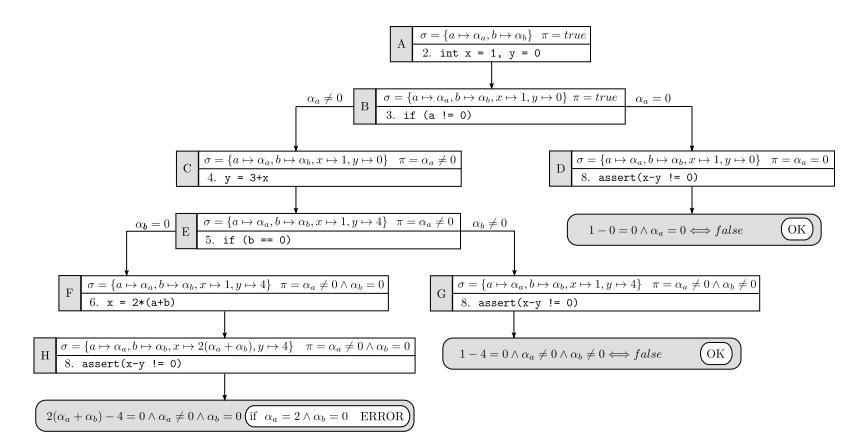
\includegraphics[scale=0.7,angle =270]{Batoev/images/sym_ex_tree.jpg}
\caption{Дерево символьного исполнения функции из листинга~\ref{baldoni_listing} работы~\cite{baldoni2018survey}}
\label{exec-tree}
\end{figure}
На этом рисунке каждый лист соответствует результату выполнения функции на любом конкретном наборе переменных, удовлетворяющем формуле этого листа $\pi$.

\subsection{Алгоритм символьного исполнения}
На листинге~\ref{alg_kuznetsov} представлен алгоритм символьного исполнения языка, содержащего четыре инструкции, из работы~\cite{kuznetsov2012efficient}.
\begin{enumerate}
    \item Алгоритм оперирует с рабочим множеством состояний $W$. Каждую итерацию цикла \smartref{alg_kuznetsov}{pickNext} из него при помощи функции $pickNext$ извлекается новое состояние для интерпретации.
    \item Процедура $ExecuteInstruction$ на листинге~\ref{execute_instruction} обрабатывает конструкции языка и получают множество следующих состояний $S$.
        \begin{itemize}
            \item Для ``присваивания'' создается новое состояние, у которого метка инструкции следует за $l$, условие пути остается неизменным, а новое отображение $s$ 
            сопоставляет переменной $v$ символьное выражение, равное $e$, вычисленному при помощи текущего отображения $s$.
            \item Конструкция ``ветвления'' проверяет возможности принятия/непринятия перехода по условию. В случае принятия создается новое состояние, у которого метка инструкция --- $l'$, условие пути --- конъюнкция старого условия и выражения $e$, а отображение $s$ остается неизменным. Аналогично, в случае непринятия к множеству $S$ добавляется состояние, у которого метка инструкции --- это следующая инструкция, а условие пути --- конъюнкция текущего условия пути с отрицанием $e$.
            \item Оператор <<assert>> задает инварианты программы \smartref{execute_instruction}{executeInsOriginalAlgoAssert}. Если инвариант не нарушен, то создается новое состояние, у которого номер инструкции --- это следующая инструкция.
            \item Оператор <<halt>> означает, что текущее состояние приводит к завершению интерпретируемой программы.
        \end{itemize}
    % Присваивание (строка 5) получает новое состояние, у которого естественным образом изменяется отображения и номер
    \item Процедура $Join$ на листинге~\ref{join} отвечает за обновление множества состояний $W$, а именно, ищутся эквивалентные состояния для объединения в одно. Хорошо известны два подхода для стратегии слияния состояний. 
    % Известно, что существуют две крайности в отношении стратегии слияния состояний.
    \begin{itemize}
        \item Никогда не сливать состояния. Данный подход называется \emph{динамическим символьным исполнением}. Плюс данного подхода --- это относительно простая для решателя ограничений формула условия пути. В свою очередь, минусом является экспоненциальный рост рабочего множества $W$.
        \item Всегда сливать состояния, если у них одинаковые метки инструкций $l$. Этот подход носит название \emph{статического символьного исполнения}. Он решает проблему роста множества состояний. Однако структура полученного после слияния состояния усложняется, затрагивая как условие пути, так и отображение $s$ и затрудняя работу решателя ограничений.
    \end{itemize}
\end{enumerate}

% \pagebreak
\begin{algorithm}
    \caption{Адаптированная схема символьного исполнения из работы~\cite{kuznetsov2012efficient}} \label{alg_kuznetsov}
\begin{algorithmic}[1]
    \Procedure{\textsc{Exec}}{}
        \State $W \gets \{(l_0, true, \lambda v.v)\}$
        \While{$W\neq\emptyset$}
            \State $(l,pc,s) \gets \textsc{pickNext}(W)$ \label{pickNext}
            \State \text{\textbf{//} Символьно исполним следующую инструкцию}
            \State $S \gets \textsc{ExecuteInstruction}(l, pc, s)$
            \State \text{\textbf{//} Объединим состояния с эквивалентными из множества $W$}
            \For{$(l', pc', s') \in S$}
                \State $W \gets \textsc{Join}(W, (l',pc',s'),\sim)$
            \EndFor
        \EndWhile
        \State \text{\texttt{print} ``no errors''}\;
    \EndProcedure
\end{algorithmic}
\end{algorithm}

\begin{algorithm}[H]
    \caption{Процедура $\textsc{Join}$ добавления нового состояния в рабочее множество} \label{join}
\begin{algorithmic}[1]
	% \Input{Рабочее множество $W$, номер инструкции $l'$, условие пути $pc'$, отображение переменных в символьные значения $s'$}
	% \Output{Новое рабочее множество $W$.}
    \Procedure{\textsc{Join}}{$W$ : states set, $l'$ : Vertex, $s'$ : Mapping}
        \If{$\exists (l', pc'', s'') \in W : (l', pc'', s'') \sim (l', pc', s')$}
            \State $W \gets W \setminus \{(l',pc'',s'')\}$
            \State $W \gets W \cup \{(l',pc' \lor pc'', Merge(pc',pc'',s', s''))\}$
        \Else
            \State $W \gets W \cup \{(l', pc', s')\}$
        \EndIf

        \State \Return W 
    \EndProcedure
\end{algorithmic}
\end{algorithm}

% \pagebreak
\begin{algorithm}[H]
    \caption{Процедура \textsc{ExecuteInstruction} символьного исполнения инструкции языка} 
    \label{execute_instruction}
\begin{algorithmic}[1]
	% \Input{Номер инструкции $l$, условие пути $pc$, отображение переменных в символьные значения $s$}
	% \Data{Множество следующих состояний $S$.}
% 	\Output{Найденные ошибки}
    \Procedure{\textsc{ExecuteInstruction}}{$l$ : Vertex, $pc$ : pathCondition, $s$ : Mapping}
        \State $S \gets \emptyset$
        \Switch{$instr(l)$}
            \Case{\textsc{\texttt{$v$ := $e$}}\qquad \texttt{// присваивание}}
                \State $S \gets \{(succ(l),pc,s[v\mapsto \cseeval{s}{e}])\}$
            \EndCase

            \Case{$if(e)$ goto $l'$ \qquad \texttt{// условный переход}}
                \If{$SAT(s, pc \land e)$}
                    \State $S \gets \{(l', pc \land e, s)\}$
                \EndIf

                \If{$SAT(s, pc \land \neg e)$}
                    \State $S \gets S\cup\{(succ(l), pc \land \neg e, s)\}$
                \EndIf
            \EndCase

            \Case{$assert(e)$ \qquad \texttt{// проверка}} \label{executeInsOriginalAlgoAssert}
                \If{$SAT(s, pc \land \neg e)$} 
                    \State abort
                \Else
                    \State $S \gets \{(succ(l),pc,s)\}$
                \EndIf
            \EndCase 

            \Case{halt\qquad \texttt{// завершение программы}}
                \State \texttt{print $pc$ }
            \EndCase
        \EndSwitch

        \State \Return S
    \EndProcedure
\end{algorithmic}
\end{algorithm}


\subsection{Композициональность}
Представим ситуацию, когда одна и та же функция вызывается несколько раз.
Конечно, можно было бы каждый раз исполнять код функции заново на переданных ей аргументах. 
Однако такой подход может быть неоправданным, если функция большая, и в общем случае неприменимым, 
если функция содержит вызов функции, находящейся в стеке вызовов, ввиду неограниченной рекурсии.  

Альтернативный способ обработки вызова функции --- это сначала исследовать функцию без предположений на входные аргументы
и получать результат, описывающий ее полное поведение, а затем <<уточнять>> результат для переданных аргументов.
Данный способ называется \emph{композициональным}, а <<уточнение>> результата производится с помощью операции \emph{композиции}.

Продемонстрируем идею операции композиции на примере (см. листинг~\ref{compositional}). Основная функция g два раза 
вызывает функцию f. Сначала исполним функцию f в <<изоляции>> и получим результат:

$res_f = \begin{cases} x \bmod 2 = 0, x \\ x \bmod 2 \neq 0, 2*x
         \end{cases}
$

% \pagebreak
Затем применим данный результат к вызовам $f$ внутри функции $g$.
Значение для переменной $b$ вычислится как композиция состояния, содержащего значение аргумента $x$, и результата функции $f$:
$$ \{ x \ra 5 \} \circ res_f = 10$$
Аналогично, получаем значение переменной $c$:
$$ \{ x \ra 10 \} \circ res_f = 10$$
\begin{lstlisting}[language={[Sharp]C}, caption={Программа для иллюстрации композиционального подхода},captionpos=b,label={compositional}]
int f(int x) {
    if (x % 2 == 0) return x;
    return 2*x;
}

int g()
{
    int b = f(5);
    int c = f(b);
    return b + c;
}
\end{lstlisting}

\subsection{Композициональные символьные кучи}
В работе \emph{<<Кучи как чистые функции: композициональное символьное исполнение без раскрутки>>} 
был введен формализм \emph{композициональной символьной памяти}. Чтобы сделать подход применимым к рекурсивным программам, \emph{символьные кучи} были расширены до  \emph{обобщённых символьных куч}. 

\begin{align*}
    Heap ::=\,\,&\heapset \cr
            \mid\,\,&\GMerge{\pair{guard}{Heap}^*} \cr
            \mid\,\,&\GMutate{Heap}{\heapset} \cr
            \mid\,\,&\GCompose{Heap}{Heap} \cr
            \mid\,\,&\GApp{func} \cr
            \mid\,\,&\GRec{\funcid} \cr
\end{align*}

$\heapset$ представляет стандартную \emph{символьную кучу}, тогда как другие варианты~--- \emph{символы куч}, которые затем будут транслированы в дизъюнкты Хорна для решения ограничений пути. 

Для данной работы необходимо расширить конструктор символа $\GRec{\funcid}$ на случай $\GRec{\id}$, где $id$ может стать идентификатором цикла внутри функции. В таком случае для трансляции в дизъюнкты Хорна необходимо получать тело идентификатора $\body{\id}$, которое содержит символьную кучу, описывающую поведение цикла в <<изоляции>>.
